\pdfoutput=1
\documentclass[12pt,a4paper]{article}

% Essential packages for analytical mechanics papers
\usepackage[utf8]{inputenc}
\usepackage[T1]{fontenc}
\usepackage{amsmath}        % Advanced math typesetting
\usepackage{amssymb}        % Mathematical symbols
\usepackage{amsfonts}       % Mathematical fonts
\usepackage{amsthm}         % Theorem environments
\usepackage[protrusion=true,expansion=false]{microtype}  % Microtypography
% \usepackage{physics}      % Physics notation - install with: tlmgr install physics
% \usepackage{mathtools}    % Extensions to amsmath - install with: tlmgr install mathtools
% \usepackage{tensor}       % Tensor notation - install with: tlmgr install tensor
% \usepackage{bm}           % Bold math symbols - install with: tlmgr install bm

% Graphics and figures
\usepackage{graphicx}
\usepackage{float}
\usepackage{caption}
\usepackage{subcaption}
\usepackage{xcolor}
\usepackage{tikz}

% Page layout
\usepackage[margin=1in]{geometry}

% References and citations
\usepackage[numbers]{natbib}
\bibliographystyle{unsrtnat}

% Hyperlinks (load last)
\usepackage[colorlinks=true,linkcolor=blue,citecolor=blue,urlcolor=blue]{hyperref}

% Theorem-like environments
\newtheorem{theorem}{Theorem}[section]
\newtheorem{lemma}[theorem]{Lemma}
\newtheorem{proposition}[theorem]{Proposition}
\newtheorem{corollary}[theorem]{Corollary}
\theoremstyle{definition}
\newtheorem{definition}[theorem]{Definition}
\theoremstyle{remark}
\newtheorem{remark}[theorem]{Remark}

\newcommand{\qq}{q_1 q_2}
\newcommand{\rdot}{\dot{r}}
\newcommand{\ddotr}{\ddot{r}}
\newcommand{\rhat}{\hat{r}}
\newcommand{\action}{\mathcal{S}}       % Action
\newcommand{\gencoord}{q}               % Generalized coordinate
\newcommand{\genvel}{\dot{q}}           % Generalized velocity
\newcommand{\genmom}{p}                 % Generalized momentum

% ===================== REVIEW MARKUP (temporary) =====================
\usepackage[most]{tcolorbox}
\tcbuselibrary{breakable,skins}
\usepackage{soul}

\definecolor{oldbg}{RGB}{255,238,240}
\definecolor{oldink}{RGB}{179,29,42}
\definecolor{newbg}{RGB}{230,255,237}
\definecolor{newink}{RGB}{26,109,52}
\definecolor{barink}{RGB}{60,66,74}
\definecolor{sigbg}{RGB}{255,221,87}
\definecolor{addbg}{RGB}{200,247,197}
\definecolor{delbg}{RGB}{255,215,215}

% Paired old/new block. #1 = change id, #2 = short caption.
\newtcolorbox{diffbox}[2]{%
  enhanced, breakable,
  colback=oldbg,
  colbacklower=newbg,
  colframe=barink,
  boxrule=0.5pt,
  arc=2pt,
  left=7pt, right=7pt, top=5pt, bottom=5pt,
  coltitle=white,
  fonttitle=\sffamily\bfseries\footnotesize,
  title={\makebox[1.9em][l]{#1}#2},
  segmentation style={draw=barink!55, dashed, line width=0.5pt},
}

% Single-sided variants for pure additions / pure removals.
\newtcolorbox{addbox}[2]{%
  enhanced, breakable,
  colback=newbg, colframe=newink, boxrule=0.5pt, arc=2pt,
  left=7pt, right=7pt, top=5pt, bottom=5pt,
  coltitle=white, fonttitle=\sffamily\bfseries\footnotesize,
  title={\makebox[1.9em][l]{#1}#2},
}

\newcommand{\oldtag}{{\sffamily\bfseries\footnotesize
  \textcolor{oldink}{$\ominus$~REMOVED \textnormal{\textmd{— paper v1.2 (current \texttt{main})}}}}\par\smallskip}
\newcommand{\newtag}{{\sffamily\bfseries\footnotesize
  \textcolor{newink}{$\oplus$~ADDED \textnormal{\textmd{— paper v1.3 (this PR)}}}}\par\smallskip}

% Inline prose markup. soul's \hl breaks across lines; \colorbox cannot.
% Fragile bits (math, \eqref, \texttt) must be \mbox-protected inside \dins.
\sethlcolor{addbg}
\newcommand{\dins}[1]{\hl{#1}}
\newcommand{\ddel}[1]{{\color{oldink}\st{#1}}}

% Highlight a single changed token inside math (sign flips).
\newcommand{\sgn}[1]{\mathbin{\colorbox{sigbg}{$#1$}}}
\newcommand{\sgnc}[1]{{\colorbox{sigbg}{$#1$}}}
\newcommand{\wchg}[1]{\colorbox{sigbg}{#1}}

\newcommand{\eqnote}[1]{\par\smallskip{\footnotesize\sffamily\textcolor{barink}{#1}}\par}
% =====================================================================

% Document metadata
\title{Computational Weber electrodynamics: symplectic n-body integration\\[4pt]{\large\sffamily\bfseries\color{oldink}[\,REVIEW COPY \textemdash\ v1.2\,$\rightarrow$\,v1.3 diff\,]}}
\author{Samer Al Duleimi \\
\small samerweb3@gmail.com}
\date{March 2026}

\begin{document}

\maketitle

\begin{abstract}
    We present the numerical simulation of $n$-body systems in Weber's electrodynamics. We derive the general Hamiltonian and equations of motion for $n$ particles and apply a symplectic integrator for non-separable Hamiltonians. Conserved quantities including energy, linear momentum, and angular momentum are verified numerically. This framework enables systematic exploration of alternative electrodynamic models for radiation and bound states of like charges below Weber's critical radius.
\end{abstract}

\begin{center}
\begin{tcolorbox}[enhanced, width=\textwidth, colback=barink!6, colframe=barink,
  boxrule=1pt, arc=3pt, left=12pt, right=12pt, top=10pt, bottom=10pt]
\begin{center}
{\sffamily\bfseries\large REVIEW COPY — NOT FOR DISTRIBUTION}\\[3pt]
{\sffamily\small Paper v1.2 $\rightarrow$ v1.3 \quad$\cdot$\quad
canonical Weber Hamiltonian correction \quad$\cdot$\quad PR \#92}
\end{center}
\smallskip
\small
Every mathematical change is shown inline as a paired block: the
\textcolor{oldink}{\textbf{removed v1.2 content on a red field}} sits directly above the
\textcolor{newink}{\textbf{added v1.3 content on a green field}}, separated by a dashed rule.
Unchanged text is left exactly as it appears in the paper, so this document still reads
as the paper itself. Equation numbering follows v1.3; blocks quoted from v1.2 are
deliberately unnumbered so they cannot be mistaken for live equations.

\smallskip
\noindent
\begin{tabular}{@{}ll@{}}
\colorbox{sigbg}{$+$} & a single token that flipped sign or changed value \\
\dins{added text} & prose inserted in v1.3 \\
\ddel{removed text} & prose deleted from v1.2 \\
\end{tabular}
\end{tcolorbox}
\end{center}

\subsection*{Index of changes}

\noindent\small
\begin{tabular}{@{}p{2.2em}p{9.2cm}p{4.1cm}@{}}
\textbf{ID} & \textbf{What changed} & \textbf{Kind} \\[2pt]
\hline\\[-6pt]
C1  & The $v \to p/m$ substitution sentence, replaced by the canonical momentum $\vec p_i = \partial L/\partial \vec v_i$ & \textbf{root error} \\
C2  & Qualifier after \texttt{h\_box}: $H = T+U$ is velocity-space energy & prose added \\
C3  & Conservation clause points at the canonical form too & prose edit \\
C4  & \texttt{alpha\_x} lead-in re-contextualised & prose edit \\
C5  & \texttt{xdot\_two}, \texttt{xdot\_two\_p2} & \textbf{sign flip} $\times 2$ \\
C6  & \texttt{pdot\_two} & \textbf{sign flip} $\times 2$ \\
C7  & Two-particle scalar inverse \texttt{radial\_inverse} & equation added \\
C8  & \texttt{hamiltonian}: $H_n \to E_n$, plus \texttt{velocity\_recovery}, \texttt{radial\_system}, \texttt{hamiltonian\_canonical} & \textbf{relabel + 3 added} \\
C9  & \texttt{xdot\_expanded}, \texttt{pdot\_expanded} & \textbf{sign flip} $\times 3$ \\
C10 & Complexity analysis & rewritten \\
C11 & Non-separability term & equation replaced \\
C12 & Appendix A momenta block & \textbf{6 equations corrected} \\
\end{tabular}

\bigskip
\noindent\small\textit{Unchanged and verified: abstract; \texttt{potential}; \texttt{force};
\texttt{ke}; $S$; $L = T-S$; \texttt{euler\_lagrange}; \texttt{H\_def}; \texttt{H};
\texttt{h\_box}; \texttt{xdot}; \texttt{pdot}; \texttt{z}; \texttt{update\_step\_x/p};
\texttt{Z}; \texttt{AZ}; \texttt{map}; \texttt{Phi}; the Newton iteration; the Discussion;
Appendix A.1 radial-acceleration identities; bibliography.}

\clearpage


\section{Introduction}

The two main equations in Weber's electrodynamics are the \textit{velocity-dependent potential}

\begin{equation}\label{potential}
    U = \frac{\qq}{r}\bigg(1 - \frac{\rdot^2}{2c^2}\bigg)
\end{equation}

and \textit{Weber's force law}

\begin{equation}\label{force}
    \vec{F}_{12} = \qq \frac{\hat{r}}{r^2}\bigg(1 - \frac{\rdot^2}{2c^2} + \frac{r\ddot{r}}{c^2}\bigg)
\end{equation}

where $q_1$ and $q_2$ are the electric charges of the two particles, $\vec{F}_{12}$ is the force on $q_1$ due to $q_2$, $r$ is the relative distance between the two particles, $\rdot = dr/dt$ is the relative radial velocity, $\ddot{r} = d\rdot/dt$ is the relative radial acceleration, and $c$ is the speed of light in vacuum. This setup is described in more detail in Appendix~\ref{app:notation} and follows conventions used in \citep{assis-weber}.

In SI units,~\eqref{potential} and~\eqref{force} would have a factor of $1/(4\pi \epsilon_0)$ multiplying the right-hand side, where $\epsilon_0$ is the permittivity of free space. We choose to omit this factor by using an alternative system of units that better suits our computational purposes (see Section~\ref{units}).

Weber's electrodynamics is an \textit{action-at-a-distance} theory. It satisfies Newton's third law of motion in the \textit{strong form} and thus $\vec{F}_{21} = -\vec{F}_{12}$ is true in general. Therefore, energy, linear momentum, and angular momentum are always conserved. Weber's force law~\eqref{force} generalizes Coulomb's law for electrostatics to include \textit{velocity-dependent} (magnetic) and \textit{acceleration-dependent} (induction) forces. This general setup has a significant \textit{computational advantage} compared to Maxwell-Heaviside's field formalism together with the Lorentz force law. We also have $\vec{F}_1 = m_1\vec{a}_1$ and $\vec{F}_2 = m_2\vec{a}_2$, where $m_1$ and $m_2$ are the \textit{inertial masses} of the particles and $\vec{a}_1$ and $\vec{a}_2$ are their accelerations with respect to an \textit{inertial frame of reference}. We adopt the \textit{Universal material frame of reference} described in Relational Mechanics \citep{assis-relational-mechanics} as our inertial reference frame.

Helmholtz argued in the 19th century that Weber's model violates the \textit{principle of conservation of energy} (see \citep{assis-weber-vol4}). Weber replied with great detail to these claims and proved energy conservation extensively in his 6th and 7th memoirs \citep{assis-weber-vol4}. Weber proved that his force~\eqref{force} can be derived from the potential~\eqref{potential}. Therefore, this force is conservative and the work done is path-independent. The Euler-Lagrange formalism indicates that Weber's electrodynamics is consistent with the principles of mechanics (see equation~\eqref{euler_lagrange}). Nowadays, Weber's electrodynamics is said to be valid only for small velocities (\textit{quasi-static approximation}) compared to $c$ and is not suitable for describing electromagnetic radiation. This might be the biggest point of critique against Weber's electrodynamics. Yet, the third term (acceleration-dependent term) in~\eqref{force} naturally falls off as $1/r$, leaving the door open for alternative theories of radiation.

To test the strengths and weaknesses of Weber's electrodynamics, we implement a \textit{symplectic numerical integrator} for investigating $n$-body systems of charged particles~\citep{WeberElectrodynamics.jl}. This allows us to explore the dynamics of charged particles interacting via Weber's force law~\eqref{force} in various configurations and scenarios. Important aspects like energy, linear momentum, and angular momentum conservation can be verified numerically. Furthermore, it paves the way for studying complex systems with oscillatory behavior and wave phenomena within the context of Weber's electrodynamics. Perhaps most interestingly, Weber's force law admits \textit{attraction between like charges} below a critical distance. We can explore the dynamics below \textit{Weber's critical radius}, which may one day lead to a purely electrodynamic planetary model of the atom \citep{assis-planetary-model}.

\section{Lagrangian and Hamiltonian formulation of Weber's electrodynamics}\label{LH}
The Lagrangian and Hamiltonian formulation of Weber's electrodynamics was introduced in 1868 by Carl Neumann (see English translation in \citep{assis-weber-vol4}). The standard formalism is described in modern notation in \citep{assis-weber}. We repeat some of the main equations and derive the general Hamiltonian and associated canonical equations for $n$ particles.

Consider a system of two particles with charges $q_1$ and $q_2$ and inertial masses $m_1$ and $m_2$. The total kinetic energy of this system is:

\begin{equation}\label{ke}
    T = m_1 \frac{\vec{v}_1 \cdot \vec{v}_1}{2} + m_2 \frac{\vec{v}_2 \cdot \vec{v}_2}{2}
\end{equation}

where $\vec{v}_1 = (\dot{x}_1, \dot{y}_1, \dot{z}_1)$ and $\vec{v}_2 = (\dot{x}_2, \dot{y}_2, \dot{z}_2)$ are the velocities of particles 1 and 2 with respect to our \textit{Universal material frame of reference}.

To define the Lagrangian, we first introduce an expression nearly identical to~\eqref{potential} but with a positive sign in front of the velocity-dependent term:

\begin{equation}
    S = \frac{\qq}{r}\bigg(1 + \frac{\rdot^2}{2c^2}\bigg)
\end{equation}

The Lagrangian is then defined as:

\begin{equation}
    \boxed{L = T - S}
\end{equation}

Although the following expression is not directly relevant for our goals, it is worth noting that we can apply the Euler-Lagrange equation to obtain the force~\eqref{force} for particle 1 in the $x$-direction by differentiating w.r.t. particle 1's position $x_1$ and velocity $\dot{x}_1$ (see Appendix~\ref{app:notation} for the notation).

\begin{equation}\label{euler_lagrange}
    F_{12}^x = \frac{d}{dt}\frac{\partial S}{\partial \dot{x}_1} - \frac{\partial S}{\partial x_1} = \qq \frac{(x_1 - x_2)}{r_{12}^3} \left(1 - \frac{\dot{r}^2}{2c^2} + \frac{r\ddot{r}}{c^2}\right)
\end{equation}

with analogous equations for particle 2 and for the $y$ and $z$ directions.

\subsection{Hamiltonian for 2 particles}
The Hamiltonian, by definition, is derived from the Lagrangian. For two particles in three spatial dimensions, it is given by

\begin{equation}\label{H_def}
    H = \sum_{i=1}^{2} \left(\dot{x}_i \frac{\partial L}{\partial \dot{x}_i} + \dot{y}_i \frac{\partial L}{\partial \dot{y}_i} + \dot{z}_i \frac{\partial L}{\partial \dot{z}_i}\right) - L
\end{equation}

This Hamiltonian is a function of individual particle \textit{positions} and \textit{velocities} in three spatial dimensions.

\begin{equation}
    H = H(x_1, y_1, z_1, x_2, y_2, z_2, \dot{x}_1, \dot{y}_1, \dot{z}_1, \dot{x}_2, \dot{y}_2, \dot{z}_2)
\end{equation}

Expanding and simplifying~\eqref{H_def} yields the Hamiltonian for two charged particles in Weber's electrodynamics.

\begin{equation}\label{H}
    H = m_1 \frac{\vec{v}_1 \cdot \vec{v}_1}{2} + m_2 \frac{\vec{v}_2 \cdot \vec{v}_2}{2} + \frac{\qq}{r}\bigg(1 - \frac{\rdot^2}{2c^2}\bigg)
\end{equation}

or more compactly,

\begin{equation}\label{h_box}
    \boxed{H = T + U}
\end{equation}

where $T$ is given by~\eqref{ke} and $U$ is the velocity-dependent potential~\eqref{potential}. \dins{Equations~\mbox{\eqref{H}} and~\mbox{\eqref{h_box}} express the conserved energy in positions and \mbox{\textit{physical velocities}}; they become a canonical Hamiltonian only after the velocities have been eliminated as described next.}

\eqnote{\textbf{C2}\quad Prose only. Equations \texttt{H} and \texttt{h\_box} are mathematically unchanged --- $H = T+U$ was always correct \emph{in velocity space}. The qualifier makes that explicit so the reader does not carry the identity into $(q,p)$ coordinates.}

Before we can apply Hamilton's canonical equations, we express the Hamiltonian in terms of \textit{positions} and \textit{momenta}. For a system of two particles in three spatial dimensions we have

\begin{equation}
    H = H(x_1, y_1, z_1, x_2, y_2, z_2, p_{x_1}, p_{y_1}, p_{z_1}, p_{x_2}, p_{y_2}, p_{z_2})
\end{equation}

\begin{diffbox}{C1}{The root error --- canonical momentum is not $m\vec v$}
\oldtag
where each velocity component $\dot{x}_i$ in~\eqref{H} is replaced by $p_{x_i}/m_i$ and
similarly for all other velocity components.

\eqnote{This single sentence was the primary error. It asserts that the Legendre
transform can be performed by dividing momentum by mass, which is false for a
velocity-dependent Lagrangian. Every later equation in the paper inherited it.}
\tcblower
\newtag
The Lagrangian $L = T - S$ is velocity dependent through $\dot{r}$, so the canonical momentum $\vec{p}_i = \partial L / \partial \vec{v}_i$ is \textit{not} the kinetic momentum $m_i \vec{v}_i$. Carrying out the differentiation with $\partial \dot{r} / \partial \vec{v}_1 = \hat{r} = -\,\partial \dot{r} / \partial \vec{v}_2$ gives

\begin{equation}\label{canonical_momentum}
    \boxed{\vec{p}_1 = m_1 \vec{v}_1 - \vec{\alpha}, \qquad \vec{p}_2 = m_2 \vec{v}_2 + \vec{\alpha}, \qquad \vec{\alpha} \equiv \frac{q_1 q_2}{c^2}\frac{\dot{r}\,(\vec{r}_1 - \vec{r}_2)}{r^2}}
\end{equation}

The correction $\vec{\alpha}$ is purely radial and enters with opposite signs, so total momentum is unaffected: $\vec{p}_1 + \vec{p}_2 = m_1\vec{v}_1 + m_2\vec{v}_2$. Velocities are therefore eliminated in favour of momenta through~\eqref{canonical_momentum}, not by replacing each $\dot{x}_i$ with $p_{x_i}/m_i$.
\end{diffbox}

\begin{diffbox}{C4}{\texttt{alpha\_x} --- algebraically identical, re-contextualised}
\oldtag
Defining
\begin{equation*}
    \alpha_x = \frac{q_1 q_2}{c^2} \frac{\dot{r}_{12} (x_1 - x_2)}{r_{12}^2}
\end{equation*}
\eqnote{In v1.2, $\dot r_{12}$ here was implicitly the $p/m$ surrogate.}
\tcblower
\newtag
Writing the components of $\vec{\alpha}$ as
\begin{equation}\label{alpha_x}
    \alpha_x = \frac{q_1 q_2}{c^2} \frac{\dot{r}_{12} (x_1 - x_2)}{r_{12}^2}
\end{equation}
\eqnote{The formula is byte-identical. What changed is its meaning: $\dot r_{12}$ is now
the \emph{physical} radial velocity, and $\alpha_x$ is a component of the momentum
correction $\vec\alpha$ introduced in C1 rather than a free-standing definition.}
\end{diffbox}

with analogous definitions for $\alpha_y$ and $\alpha_z$, we apply Hamilton's equations~\eqref{xdot} and~\eqref{pdot} to obtain

\begin{diffbox}{C5}{\texttt{xdot\_two}, \texttt{xdot\_two\_p2} --- both signs flipped}
\oldtag
\begin{equation*}
    \dot{x}_1 = \frac{1}{m_1} \left(p_{x_1} \sgn{-} \alpha_x\right)
\end{equation*}
\begin{equation*}
    \dot{x}_2 = \frac{1}{m_2} \left(p_{x_2} \sgn{+} \alpha_x\right)
\end{equation*}
\tcblower
\newtag
\begin{equation}\label{xdot_two}
    \dot{x}_1 = \frac{1}{m_1} \left(p_{x_1} \sgn{+} \alpha_x\right)
\end{equation}

\begin{equation}\label{xdot_two_p2}
    \dot{x}_2 = \frac{1}{m_2} \left(p_{x_2} \sgn{-} \alpha_x\right)
\end{equation}
\eqnote{Solving $\vec p_1 = m_1\vec v_1 - \vec\alpha$ for $\vec v_1$ gives
$+\vec\alpha$, not $-\vec\alpha$. Note that
\texttt{theory/WeberElectrodynamics.md} already carried these signs correctly ---
the paper and the theory notes contradicted each other.}
\end{diffbox}

and

\begin{diffbox}{C6}{\texttt{pdot\_two} --- both $1/c^2$ signs flipped}
\oldtag
\begin{equation*}
    \dot{p}_{x_1} = \frac{q_1 q_2}{r_{12}^2}\left[\frac{(x_1 - x_2)}{r_{12}}\left(1 \sgn{-} \frac{3\dot{r}_{12}^2}{2 c^2}\right) \sgn{+} \frac{\dot{r}_{12}(\dot{x}_1 - \dot{x}_2)}{c^2}\right]
\end{equation*}
\tcblower
\newtag
\begin{equation}\label{pdot_two}
    \dot{p}_{x_1} = \frac{q_1 q_2}{r_{12}^2}\left[\frac{(x_1 - x_2)}{r_{12}}\left(1 \sgn{+} \frac{3\dot{r}_{12}^2}{2 c^2}\right) \sgn{-} \frac{\dot{r}_{12}(\dot{x}_1 - \dot{x}_2)}{c^2}\right]
\end{equation}
\eqnote{Both signs are consequences of the same C1 error and cannot be corrected
independently of it. \texttt{pdot\_two\_p2} ($\dot p_{x_2} = -\dot p_{x_1}$) is unchanged.}
\end{diffbox}

\begin{equation}\label{pdot_two_p2}
    \dot{p}_{x_2} = -\dot{p}_{x_1}
\end{equation}

with analogous equations for the $y$ and $z$ directions. Note that $\dot{p}_{x_1} + \dot{p}_{x_2} = 0$, but $\dot{x}_1 - \dot{x}_2 \neq 0$ in general. \dins{Throughout, \mbox{$\dot{r}_{12}$} and \mbox{$\dot{x}_1 - \dot{x}_2$} denote \mbox{\textit{physical}} velocities; \mbox{$\vec{\alpha}$} in~\mbox{\eqref{xdot_two}} and~\mbox{\eqref{xdot_two_p2}} contains \mbox{$\dot{r}$}, so these relations are implicit.}

\begin{addbox}{C7}{Two-particle scalar inverse --- new, resolves the implicitness}
\newtag
For two particles the implicit relation reduces to a single scalar equation. With $\mu = m_1 m_2/(m_1+m_2)$ the reduced mass and $p_r = \mu\,\hat{r}\cdot(\vec{p}_1/m_1 - \vec{p}_2/m_2)$ the momentum conjugate to the relative radial coordinate, contracting~\eqref{canonical_momentum} with $\hat{r}$ gives

\begin{equation}\label{radial_inverse}
    \boxed{p_r = \left(\mu - \frac{q_1 q_2}{r c^2}\right)\dot{r}, \qquad \dot{r} = \frac{p_r}{\mu - q_1 q_2/(r c^2)}}
\end{equation}

so the physical radial velocity follows in closed form from the canonical momenta. Only the relative radial motion is modified; the centre-of-mass and relative transverse momenta keep their ordinary relation to velocity. The effective radial inertia $\mu - q_1 q_2/(r c^2)$ vanishes for like charges exactly at Weber's critical radius $\rho = q_1 q_2/(\mu c^2)$, revisited in the Discussion; below $\rho$ it is negative but finite.

\eqnote{Nothing corresponds to this in v1.2, which had no notion that the
velocity--momentum relation needed inverting at all. Note $p_r = \mu\dot r$ is
recovered only as $c\to\infty$.}
\end{addbox}

\subsection{Conserved quantities and symmetries}
Weber's electrodynamics for 2 particles conserves energy, linear momentum, and angular momentum. These conserved quantities arise from symmetries in the Hamiltonian~\eqref{h_box}\dins{, equivalently the canonical form~\mbox{\eqref{hamiltonian_canonical}},} according to Noether's theorem.\footnote{\textbf{C3.} Clause added. The conservation claims themselves are unchanged and still hold; the correction preserves translation, rotation, and time-translation invariance, all of which are re-verified numerically in the PR.} The conservation of energy follows from the \textit{time-translation symmetry} of the Hamiltonian, meaning that the Hamiltonian has no explicit time dependence. The conservation of linear momentum arises from the \textit{translational symmetry} of the Hamiltonian, meaning that shifting all particle positions by a constant vector does not change the form of the Hamiltonian. The conservation of angular momentum is a consequence of the \textit{rotational symmetry} of the Hamiltonian, indicating that rotating the entire system around any axis does not change the form of the Hamiltonian. These symmetries arise from the fact that Weber's electrodynamics relies only on what Assis calls \textit{relational magnitudes} (see Appendix~\ref{app:additional-remarks}).

\subsection{Hamiltonian for \texorpdfstring{$n$}{n} particles}\label{n-body-hamiltonian}
\begin{diffbox}{C8a}{\texttt{hamiltonian} --- $H_n$ relabelled $E_n$, right-hand side identical}
\oldtag
For a system with $n$ particles, the \wchg{Hamiltonian}~\eqref{H} generalizes to:
\begin{equation*}
    \sgnc{H_n} = \sum_{i=1}^{n} \frac{1}{2} m_i v_i^2 + \sum_{i=1}^{n} \sum_{j=i+1}^{n} \frac{q_i q_j}{r_{ij}} \left(1 - \frac{\dot{r}_{ij}^2}{2 c^2}\right)
\end{equation*}
\tcblower
\newtag
For a system with $n$ particles, the \wchg{energy}~\eqref{H} generalizes to:
\begin{equation}\label{hamiltonian}
    \sgnc{E_n} = \sum_{i=1}^{n} \frac{1}{2} m_i v_i^2 + \sum_{i=1}^{n} \sum_{j=i+1}^{n} \frac{q_i q_j}{r_{ij}} \left(1 - \frac{\dot{r}_{ij}^2}{2 c^2}\right)
\end{equation}
\eqnote{The right-hand side is unchanged to the byte. It was always the
velocity-space energy; calling it a Hamiltonian and then feeding it to
Hamilton's equations in $(q,p)$ was the error. Renaming it $E_n$ frees the
symbol $H_n$ for the genuine canonical Hamiltonian added below.}
\end{diffbox}

where the double sum is taken over every unique particle pair $i$ and $j$ (see Section~\ref{complexity}). The conservation laws stated previously still hold for this general case.

\begin{addbox}{C8b}{Velocity recovery and the exact canonical Hamiltonian --- all new}
\newtag
Equation~\eqref{hamiltonian} is expressed in positions and \textit{physical velocities}. To obtain the canonical Hamiltonian we must first recover the velocities from the canonical momenta~\eqref{canonical_momentum}. Generalizing~\eqref{alpha_x} to $n$ particles, the correction to $\vec{v}_i$ is a sum over the pairs containing particle $i$,

\begin{equation}\label{velocity_recovery}
    \vec{v}_i = \frac{\vec{p}_i}{m_i} + \frac{1}{m_i}\sum_{\substack{j=1 \\ j \neq i}}^{n} k_{ij}\,\dot{r}_{ij}\,\hat{r}_{ij}, \qquad k_{ij} \equiv \frac{q_i q_j}{c^2 r_{ij}}
\end{equation}

Each $\dot{r}_{ij}$ on the right-hand side depends on the velocities themselves, so the $n(n-1)/2$ pair radial velocities must be obtained together. Contracting~\eqref{velocity_recovery} with $\hat{r}_{ab}$ gives a linear system in those unknowns,

\begin{equation}\label{radial_system}
    \dot{r}_{ab} = s_{ab} + \sum_{\substack{\text{pairs} \\ (c,d)}} G_{ab,cd}\,k_{cd}\,\dot{r}_{cd}, \qquad s_{ab} \equiv \hat{r}_{ab}\cdot\left(\frac{\vec{p}_a}{m_a} - \frac{\vec{p}_b}{m_b}\right)
\end{equation}

where $s_{ab}$ is the radial rate one would obtain by mistaking canonical momentum for kinetic momentum, and $G_{ab,cd} = (\hat{r}_{ab}\cdot\hat{r}_{cd})\left[(\delta_{ac}-\delta_{ad})/m_a - (\delta_{bc}-\delta_{bd})/m_b\right]$ couples pairs through their shared particles. With the $\dot{r}_{ij}$ in hand, the exact canonical Hamiltonian is

\begin{equation}\label{hamiltonian_canonical}
    \boxed{H_n(\mathbf{q},\mathbf{p}) = \frac{1}{2}\sum_{i=1}^{n} \vec{p}_i \cdot \vec{v}_i + \sum_{i=1}^{n}\sum_{j=i+1}^{n} \frac{q_i q_j}{r_{ij}} = \sum_{i=1}^{n} \frac{|\vec{p}_i|^2}{2 m_i} + \frac{1}{2}\sum_{i=1}^{n}\sum_{j=i+1}^{n} k_{ij}\,\dot{r}_{ij}\,s_{ij} + \sum_{i=1}^{n}\sum_{j=i+1}^{n} \frac{q_i q_j}{r_{ij}}}
\end{equation}

and $H_n(\mathbf{q},\mathbf{p}) = E_n(\mathbf{q},\mathbf{v}(\mathbf{q},\mathbf{p}))$ by the Legendre transform. In the Coulomb limit $c \to \infty$, and at any instant where every $\dot{r}_{ij}$ vanishes, $k_{ij} \to 0$ and~\eqref{hamiltonian_canonical} reduces to $\sum_i |\vec{p}_i|^2/(2m_i) + \sum_{i<j} q_i q_j / r_{ij}$.

\eqnote{v1.2 contained none of this. $s_{ij}$ is exactly the quantity v1.2 called
$\dot r_{ij}$ in $(q,p)$ coordinates --- naming it separately is what makes the
error visible. Verified symbolically for $n=2$ and by 40-digit finite differences
for $n=3$ in \texttt{verify\_formulas.py}.}
\end{addbox}

For a system of $n$ particles in one spatial dimension $x$, Hamilton's equations of motion are given by

\begin{equation}\label{xdot}
    \dot{x}_i = \frac{\partial H_n}{\partial p_{x_i}}
\end{equation}

\begin{equation}\label{pdot}
    \dot{p}_{x_i} = -\frac{\partial H_n}{\partial x_i}
\end{equation}

for particle $i \in \{1, 2, \ldots, n\}$. In three dimensions, we also have the analogous equations for $y_i$ and $z_i$.

For a system of $n$ particles,~\eqref{xdot} expands to

\begin{diffbox}{C9}{\texttt{xdot\_expanded}, \texttt{pdot\_expanded} --- three signs flipped}
\oldtag
\begin{equation*}
    \boxed{\dot{x}_i = \frac{1}{m_i} \left(p_{x_i} \sgn{-} \sum_{\substack{j=1 \\ j \neq i}}^{n} \frac{q_i q_j}{c^2} \frac{\dot{r}_{ij} (x_i - x_j)}{r_{ij}^2}\right)}
\end{equation*}
\begin{equation*}
    \boxed{\dot{p}_{x_i} = \sum_{\substack{j=1 \\ j \neq i}}^{n} \frac{q_i q_j}{r_{ij}^2}\left[\frac{(x_i - x_j)}{r_{ij}}\left(1 \sgn{-} \frac{3\dot{r}_{ij}^2}{2 c^2}\right) \sgn{+} \frac{\dot{r}_{ij}(\dot{x}_i - \dot{x}_j)}{c^2}\right]}
\end{equation*}
\tcblower
\newtag
\begin{equation}\label{xdot_expanded}
    \boxed{\dot{x}_i = \frac{1}{m_i} \left(p_{x_i} \sgn{+} \sum_{\substack{j=1 \\ j \neq i}}^{n} \frac{q_i q_j}{c^2} \frac{\dot{r}_{ij} (x_i - x_j)}{r_{ij}^2}\right)}
\end{equation}

for particle $i \in \{1, 2, \ldots, n\}$, with analogous expressions for $\dot{y}_i$ and $\dot{z}_i$, and~\eqref{pdot} expands to

\begin{equation}\label{pdot_expanded}
    \boxed{\dot{p}_{x_i} = \sum_{\substack{j=1 \\ j \neq i}}^{n} \frac{q_i q_j}{r_{ij}^2}\left[\frac{(x_i - x_j)}{r_{ij}}\left(1 \sgn{+} \frac{3\dot{r}_{ij}^2}{2 c^2}\right) \sgn{-} \frac{\dot{r}_{ij}(\dot{x}_i - \dot{x}_j)}{c^2}\right]}
\end{equation}

for particle $i \in \{1, 2, \ldots, n\}$, with analogous expressions for $\dot{p}_{y_i}$ and $\dot{p}_{z_i}$. \dins{In both boxed equations every \mbox{$\dot{r}_{ij}$} and \mbox{$\dot{x}_i - \dot{x}_j$} is a physical velocity obtained from the simultaneous system~\mbox{\eqref{radial_system}}; equation~\mbox{\eqref{xdot_expanded}} is the component form of~\mbox{\eqref{velocity_recovery}}.}
\eqnote{These are the $n$-body forms of C5 and C6 and carry the same three sign
changes. Both remain boxed as the paper's headline results.}
\end{diffbox}

Equations~\eqref{xdot_expanded} and~\eqref{pdot_expanded} together with their analogs for $y$ and $z$ directions form a system of $6n$ first-order ordinary differential equations that describe the time evolution in \textit{phase space} of an $n$-particle system for Weber's electrodynamics. For any time $t$, the \textit{state} of the system is represented by a point $\mathbf{z}$ in a $6n$-dimensional phase space

\begin{equation}\label{z}
    \mathbf{z} = (x_1, y_1, z_1, \ldots, x_n, y_n, z_n, p_{x_1}, p_{y_1}, p_{z_1}, \ldots, p_{x_n}, p_{y_n}, p_{z_n}) \in \mathbb{R}^{6n}
\end{equation}

where every component is a function of time $t$. To evolve the system in time using small discrete time steps $\Delta t$, we compute

\begin{equation}\label{update_step_x}
    x_i^{t + \Delta t} = x_i^t + \Delta t \, \dot{x}_i^t
\end{equation}
\begin{equation}\label{update_step_p}
    p_{x_i}^{t + \Delta t} = p_{x_i}^t + \Delta t \, \dot{p}_{x_i}^t
\end{equation}

and similarly for $y_i$ and $z_i$, where $\dot{x}_i^t$ and $\dot{p}_{x_i}^t$ are computed using~\eqref{xdot_expanded} and~\eqref{pdot_expanded} at time $t$. Repeating this process iteratively allows us to evolve a system of $n$ charged particles interacting via Weber's electrodynamics over time given some initial positions and momenta.

\subsection[Computational complexity of Hamiltonian Weber electrodynamics]{Computational complexity of Hamiltonian Weber \\ electrodynamics}\label{complexity}
To understand the total number of unique interactions, consider an $n \times n$ matrix where entry $(i,j)$ represents the interaction between particles $i$ and $j$:

\begin{center}
    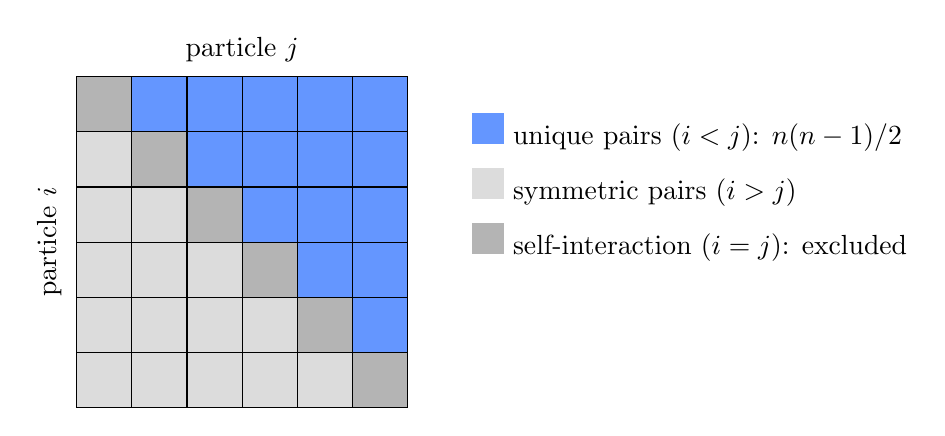
\begin{tikzpicture}[scale=0.7]
        % Define colors
        \definecolor{unique}{RGB}{100,150,255}
        \definecolor{symmetric}{RGB}{220,220,220}
        \definecolor{diagonal}{RGB}{180,180,180}

        % Draw grid for n=6 example
        \foreach \i in {0,...,5} {
                \foreach \j in {0,...,5} {
                        \pgfmathtruncatemacro{\row}{\i}
                        \pgfmathtruncatemacro{\col}{\j}

                        % Determine color based on position
                        \ifnum\row<\col
                            \fill[unique] (\j, -\i) rectangle (\j+1, -\i-1);
                        \else
                            \ifnum\row>\col
                                \fill[symmetric] (\j, -\i) rectangle (\j+1, -\i-1);
                            \else
                                \fill[diagonal] (\j, -\i) rectangle (\j+1, -\i-1);
                            \fi
                        \fi

                        % Draw grid lines
                        \draw (\j, -\i) rectangle (\j+1, -\i-1);
                    }
            }

        % Add labels
        \node at (3, 0.5) {particle $j$};
        \node[rotate=90] at (-0.5, -3) {particle $i$};

        % Add legend
        \node[anchor=west] at (7, -1) {\textcolor{unique}{\rule{0.4cm}{0.4cm}} unique pairs ($i<j$): $n(n-1)/2$};
        \node[anchor=west] at (7, -2) {\textcolor{symmetric}{\rule{0.4cm}{0.4cm}} symmetric pairs ($i>j$)};
        \node[anchor=west] at (7, -3) {\textcolor{diagonal}{\rule{0.4cm}{0.4cm}} self-interaction ($i=j$): excluded};

    \end{tikzpicture}
\end{center}

\begin{diffbox}{C10}{Complexity --- the $\mathcal{O}(n^2)$ claim was incomplete}
\oldtag
For a system of $n$ particles, we thus have a total of $n(n-1)/2$ unique particle pairs, resulting in a computational complexity of order $\mathcal{O}(n^2)$.

A naive implementation would compute all $n(n-1)$ interactions, but by exploiting~\eqref{alpha_x},~\eqref{xdot_two},~\eqref{xdot_two_p2},~\eqref{pdot_two} and~\eqref{pdot_two_p2}, we reduce this to $n(n-1)/2$ interactions.

Furthermore, each evaluation of~\eqref{xdot_expanded} and~\eqref{pdot_expanded} only needs to compute $r_{ij}$ and $\dot{r}_{ij}$ and their powers once per unique pair, which further reduces the computational load.

\eqnote{This asserted that per-pair work completes an evaluation. It does not:
with $\vec p \ne m\vec v$ the velocities are not known until a coupled system is
solved.}
\tcblower
\newtag
For a system of $n$ particles, we thus have a total of $P = n(n-1)/2$ unique particle pairs, so assembling the pair geometry costs $\mathcal{O}(n^2)$.

A naive implementation would compute all $n(n-1)$ interactions, but by exploiting~\eqref{alpha_x},~\eqref{xdot_two},~\eqref{xdot_two_p2},~\eqref{pdot_two} and~\eqref{pdot_two_p2}, we reduce this to $P$ interactions. Each evaluation of~\eqref{xdot_expanded} and~\eqref{pdot_expanded} then needs $r_{ij}$ and $\dot{r}_{ij}$ and their powers only once per unique pair.

Pair evaluation alone does not, however, complete an evaluation of the equations of motion. Because canonical momentum is not kinetic momentum, the physical velocities entering~\eqref{xdot_expanded} and~\eqref{pdot_expanded} are only available after solving the coupled system~\eqref{radial_system}, whose matrix is $P \times P$ and dense in general. A direct factorization costs $\mathcal{O}(P^3) = \mathcal{O}(n^6)$ per evaluation, so for large $n$ the linear solve, not the pair sum, dominates. Two remarks temper this. First, $\mathbb{I} - GK$ is a perturbation of the identity of order $q^2/(m c^2 r)$, so for sub-relativistic configurations a few Jacobi or conjugate-gradient iterations converge to machine precision at $\mathcal{O}(n^2)$ cost per iteration. Second, for the two-body case $P = 1$ and the solve degenerates to the closed-form division~\eqref{radial_inverse}. Our reference implementation~\citep{WeberElectrodynamics.jl} uses a direct dense factorization, which is exact at all separations and comfortably fast for the particle counts studied here.
\end{diffbox}

\subsection{Units and numerical values}\label{units}
When performing numerical computations, we often rely on the 64-bit floating-point representation of decimal numbers. This number representation introduces a trade-off between range and precision. To maintain optimal precision, it is advantageous to work with number values near the order of magnitude of 1. In Weber's electrodynamics, we are mostly interested in numerical values that are relatively small when expressed in SI units. In our numerical computations, we will convert to smaller units to obtain larger numerical values for the same physical quantities.

In the 19th century, Gauss and Weber used an absolute system of units based on the \textit{millimeter}, \textit{milligram}, and \textit{second}. This system is not to be confused with the CGS-system of units, also known as the Gaussian system of units~\citep{assis-weber-vol1}. The potential~\eqref{potential} and force~\eqref{force} were originally introduced by Weber in this absolute system of units. The units in this system for the potential~\eqref{potential} are $mg \cdot mm^2 / s^2$ and for the force~\eqref{force} are $mg \cdot mm / s^2$.

Thus, the original system of Gauss and Weber, compared to the SI system, is better suited for our computational purposes, though not sufficient. In practice, we need even smaller units like \textit{micrometer}, \textit{microgram} and \textit{microsecond} or even smaller to obtain numerical values near the order of magnitude of 1 for typical values of charge, mass and distance encountered in Weber's electrodynamics.

Another common system of units is obtained by setting $c = 1$ and (in the case of SI units) $1/(4\pi \epsilon_0) = 1$. This system is often used in computational physics for the same reasons mentioned above.

\section{Symplectic numerical integration of non-separable Hamiltonian systems}\label{symplectic}
A numerical method is called \textit{symplectic} if it preserves the \textit{phase space volume} of Hamiltonian systems over time according to \textit{Liouville's theorem}. Standard symplectic methods require the Hamiltonian to be separable into kinetic and potential energy terms that each depend only on positions or momenta. \begin{diffbox}{C11}{Non-separability --- the offending term restated}
\oldtag
The general Hamiltonian for Weber's electrodynamics~\eqref{hamiltonian} is non-separable because the velocity-dependent term
\begin{equation*}
    -\frac{\qq \dot{r}_{ij}^2}{2 c^2 r_{ij}}
\end{equation*}
is both a function of the positions and momenta after the Legendre transformation. Therefore, standard symplectic methods cannot be applied directly.
\tcblower
\newtag
The canonical Hamiltonian for Weber's electrodynamics~\eqref{hamiltonian_canonical} is non-separable because the velocity-dependent term

\begin{equation}
    \frac{1}{2} k_{ij}\,\dot{r}_{ij}\,s_{ij}
\end{equation}

is a function of both the positions and the momenta after the Legendre transformation: $k_{ij}$ and $s_{ij}$ depend on positions and momenta explicitly, and $\dot{r}_{ij}$ does so through the solve~\eqref{radial_system}. Therefore, standard symplectic methods cannot be applied directly.
\eqnote{The \emph{conclusion} --- non-separability, hence the need for the
extended-phase-space integrator --- is unchanged, so everything downstream in
Section~\ref{symplectic} (Strang splitting, symmetric projection, $\Phi$, the
Newton iteration) is mathematically untouched.}
\end{diffbox} Recent work by \citet{Pihajoki2015} and \citet{Tao2016} introduced explicit symplectic methods using the clever extended phase space method. Building on these approaches, \citet{Jayawardana2023} developed a semi-explicit symplectic integrator for non-separable Hamiltonian systems that also preserves quadratic invariants (see \citep{Ohsawa2023}). Currently, this is one of the most suitable methods for our purposes. We describe it briefly here.

We introduce compact vector notation $\mathbf{q} = (x_1, y_1, z_1, \ldots, x_n, y_n, z_n) \in \mathbb{R}^{3n}$ for positions and $\mathbf{p} = (p_{x_1}, p_{y_1}, p_{z_1}, \ldots, p_{x_n}, p_{y_n}, p_{z_n}) \in \mathbb{R}^{3n}$ for momenta, so that $\mathbf{z} = (\mathbf{q}, \mathbf{p}) \in \mathbb{R}^{6n}$ as in~\eqref{z}. The extended phase space doubles the phase space by introducing another pair of positions and momenta $\mathbf{x} \in \mathbb{R}^{3n}$ and $\mathbf{y} \in \mathbb{R}^{3n}$, giving the state vector in extended phase space

\begin{equation}\label{Z}
    \mathbf{Z} = (\mathbf{q}, \mathbf{x}, \mathbf{p}, \mathbf{y}) \in \mathbb{R}^{12n}
\end{equation}

The conditions $\mathbf{x} = \mathbf{q}$ and $\mathbf{y} = \mathbf{p}$ are equivalent to a system in the original phase space. If

\begin{equation}
    \mathbf{A} = \begin{pmatrix}
        \mathbf{I} & -\mathbf{I} & \mathbf{0} & \mathbf{0}  \\
        \mathbf{0} & \mathbf{0}  & \mathbf{I} & -\mathbf{I}
    \end{pmatrix}
\end{equation}

where $\mathbf{I}$ and $\mathbf{0}$ denote the $3n \times 3n$ identity and zero matrices, then the condition we are interested in is expressed as

\begin{equation}\label{AZ}
    \mathbf{A} \mathbf{Z} = (\mathbf{q} - \mathbf{x}, \mathbf{p} - \mathbf{y}) = 0
\end{equation}

We define a \textit{symplectic map} that updates the state vector~\eqref{Z} over a time step $\Delta t$

\begin{equation}\label{map}
    \Phi_{\Delta t}: \mathbf{Z}_t \mapsto \mathbf{Z}_{t+\Delta t}
\end{equation}

Using the update steps~\eqref{update_step_x} and~\eqref{update_step_p} to compute~\eqref{xdot_expanded} and~\eqref{pdot_expanded} for $(\mathbf{q}, \mathbf{p})$ and $(\mathbf{x}, \mathbf{y})$ separately, we can evolve the system in the extended phase space by defining two separate flows $\Phi^A_{\Delta t}$ and $\Phi^B_{\Delta t}$ that we apply in this order

\begin{itemize}
    \item $\Phi^A_{\Delta t / 2}$ evolves $(\mathbf{x}, \mathbf{p})$ from $t$ to $t + \Delta t / 2$, using the values of $(\mathbf{q}, \mathbf{y})$ at time $t$
    \item $\Phi^B_{\Delta t}$ evolves $(\mathbf{q}, \mathbf{y})$ from $t$ to $t + \Delta t$, using the values of $(\mathbf{x}, \mathbf{p})$ at time $t + \Delta t / 2$
    \item $\Phi^A_{\Delta t / 2}$ evolves $(\mathbf{x}, \mathbf{p})$ from $t + \Delta t / 2$ to $t + \Delta t$, using the values of $(\mathbf{q}, \mathbf{y})$ at time $t + \Delta t$
\end{itemize}

Our mapping~\eqref{map} becomes

\begin{equation}\label{Phi}
    \boxed{\Phi_{\Delta t} = \Phi^A_{\Delta t/2} \circ \Phi^B_{\Delta t} \circ \Phi^A_{\Delta t/2}}
\end{equation}

This staggered update scheme is referred to as \textit{Strang splitting} (also known as the \textit{leapfrog} method), which is a second-order symplectic integrator.

The key innovation of \citep{Jayawardana2023} is the \textit{symmetric projection method}, which applies a carefully chosen \textit{shift vector} $\boldsymbol{\mu} \in \mathbb{R}^{6n}$ before and after the explicit evolution step~\eqref{Phi} to ensure~\eqref{AZ}.

The full computation can then be succinctly expressed as a non-linear equation

\begin{equation}
    \mathbf{f}(\boldsymbol{\mu}) = \mathbf{A} (\Phi_{\Delta t}(\mathbf{Z}_n + \mathbf{A}^T \boldsymbol{\mu}) + \mathbf{A}^T \boldsymbol{\mu}) = 0
\end{equation}

where the solution satisfies~\eqref{AZ}. One can solve this equation iteratively using Newton's method. Starting from an initial guess $\boldsymbol{\mu}_{(0)} = 0$, we compute successive approximations using the \textit{simplified Newton approximations} (see \citep{Jayawardana2023} and \citep{Hairer2006})

\begin{equation}
    \boldsymbol{\mu}_{(k+1)} = \boldsymbol{\mu}_{(k)} - \frac{1}{4} \mathbf{f}(\boldsymbol{\mu}_{(k)})
\end{equation}

where $k$ is the iteration index. We repeat this process until

\begin{equation}
    ||\boldsymbol{\mu}_{(k+1)} - \boldsymbol{\mu}_{(k)}|| < \epsilon
\end{equation}

where $\epsilon$ is a small tolerance value.

The full specification of this semi-explicit symplectic integrator can be found in \citep{Jayawardana2023}. We have implemented this integrator in the Julia programming language. For examples, ongoing work, and numerical validation including energy conservation benchmarks and convergence studies, see \citep{WeberElectrodynamics.jl}.

\section{Discussion}

The computational framework presented in this paper enables the numerical simulation of $n$-body systems governed by Weber's electrodynamics. Beyond validating conservation laws, this framework opens the door to simulating electronic systems entirely from first principles using a direct particle-interaction model rather than field-based methods. The acceleration-dependent term in Weber's force~\eqref{force} falls off as $1/r$. This naturally suggests radiation-like phenomena that are cumbersome to simulate within standard Maxwellian field theory, which has been shown to be inconsistent \citep{vlaenderen2016}.

We could in principle also simulate \textit{the physics} of passive analog components such as coils, capacitors, and transformers by considering charged particles and their mutual motion. To move in this direction, we need to consider the role of \textit{surface charges on resistive conductors} (see \citep{jackson1996} and \citep{assis-electric-force}). Self-inductance in coils and mutual inductance in transformers can be simulated by considering the correct inductance calculations presented in \citep{assis-inductance}. It is also relevant to note the \textit{Amperian current element}, an electrically neutral system of two opposite (not necessarily equal) charges moving in opposite directions, which can be used to model electric currents \citep{assis-ampere}.

Perhaps the most promising direction for future research lies in the remarkable fact that Weber's force law admits \textit{attraction between like charges} below a critical separation $\rho = q_1 q_2/(\mu c^2)$, where $\mu = m_1 m_2 / (m_1 + m_2)$ is the reduced mass. At this critical radius, the sign of the force between $q_1$ and $q_2$ is reversed. For $r < \rho$, the particles respond to the still-repulsive Coulomb force as if they had ``negative inertia'', accelerating toward each other rather than away. Weber himself identified this phenomenon in his Sixth Memoir (1871)~\citep{assis-weber-vol4}.

\citet{Frauenfelder2024} have shown that classical collisions at the origin are regularizable only when the angular momentum $\ell = 0$, corresponding to purely radial (head-on) motion. For $\ell \neq 0$, the system is not regularizable. This constraint poses a fundamental challenge: finding stable, bound configurations of like charges below the critical radius that go beyond purely radial oscillation. One avenue is to develop advanced regularization or stabilization techniques that could handle the $\ell \neq 0$ singularity. Another, perhaps more promising, approach is to expand our view beyond the isolated two-body problem and consider multi-particle systems. For instance, we could balance a pair of like charges in the sub-critical regime with oppositely charged particles above $\rho$, or explore other conceivable configurations whose mutual interactions provide the stabilizing forces that a single pair lacks.

This line of investigation is part of a long-standing program that originated with Weber himself and his planetary model of the atom (see \citep{assis-planetary-model} and \citep{assis-weber-vol4}), in which bound pairs of like charges form atomic nuclei while unlike charges orbit under the combined electrodynamic forces. With the computational tools presented here, and with modern AI-assisted methods that can efficiently search the space of possible configurations, we can explore this vast landscape of possibilities more thoroughly than was previously feasible. We could in principle automate algebraic manipulations and systematic testing. The ultimate goal of this program is to uncover the electrodynamic origins of the periodic table of elements.

\appendix

\section{Notation and relational magnitudes}\label{app:notation}
For a system of two particles, we define the following quantities. Particle 1 and particle 2 have electric charges $q_1, q_2$ and inertial masses $m_1, m_2$. In the Gauss-Weber system of units, charge has units of $\sqrt{mg \cdot mm^3 / s^2}$.

The individual particle positions, velocities, and accelerations are

\begin{align*}
    \vec{r}_1 = (x_1, y_1, z_1)                      &  & \vec{r}_2 = (x_2, y_2, z_2)                      \\
    \vec{v}_1 = (\dot{x}_1, \dot{y}_1, \dot{z}_1)    &  & \vec{v}_2 = (\dot{x}_2, \dot{y}_2, \dot{z}_2)    \\
    \vec{a}_1 = (\ddot{x}_1, \ddot{y}_1, \ddot{z}_1) &  & \vec{a}_2 = (\ddot{x}_2, \ddot{y}_2, \ddot{z}_2)
\end{align*}

\begin{diffbox}{C12}{Appendix A momenta --- all six equations corrected}
\oldtag
The individual particle momenta are
\begin{align*}
    p_{x_1} = m_1 \dot{x}_1 &  & p_{x_2} = m_2 \dot{x}_2 \\
    p_{y_1} = m_1 \dot{y}_1 &  & p_{y_2} = m_2 \dot{y}_2 \\
    p_{z_1} = m_1 \dot{z}_1 &  & p_{z_2} = m_2 \dot{z}_2
\end{align*}
\eqnote{The notation appendix stated the error as a definition, which is why it
propagated so cleanly through the rest of the paper.}
\tcblower
\newtag
The individual particle canonical momenta are given by~\eqref{canonical_momentum}, componentwise

\begin{align*}
    p_{x_1} = m_1 \dot{x}_1 \sgn{-} \alpha_x &  & p_{x_2} = m_2 \dot{x}_2 \sgn{+} \alpha_x \\
    p_{y_1} = m_1 \dot{y}_1 \sgn{-} \alpha_y &  & p_{y_2} = m_2 \dot{y}_2 \sgn{+} \alpha_y \\
    p_{z_1} = m_1 \dot{z}_1 \sgn{-} \alpha_z &  & p_{z_2} = m_2 \dot{z}_2 \sgn{+} \alpha_z
\end{align*}

with $\alpha_x$, $\alpha_y$, $\alpha_z$ the components of $\vec{\alpha}$ defined in~\eqref{alpha_x}. The kinetic momenta $m_i \dot{x}_i$ are recovered only when $\dot{r} = 0$ or in the limit $c \to \infty$.
\end{diffbox}

The relative positions, velocities, and accelerations between particle 1 and particle 2 are

\begin{alignat*}{3}
    x & = x_1 - x_2 \qquad & \dot{x} & = \dot{x}_1 - \dot{x}_2 \qquad & \ddot{x} & = \ddot{x}_1 - \ddot{x}_2 \\
    y & = y_1 - y_2 \qquad & \dot{y} & = \dot{y}_1 - \dot{y}_2 \qquad & \ddot{y} & = \ddot{y}_1 - \ddot{y}_2 \\
    z & = z_1 - z_2 \qquad & \dot{z} & = \dot{z}_1 - \dot{z}_2 \qquad & \ddot{z} & = \ddot{z}_1 - \ddot{z}_2
\end{alignat*}

The relative position, velocity, and acceleration vectors are

\[\vec{r} = (x, y, z)\]
\[\vec{v} = (\dot{x}, \dot{y}, \dot{z})\]
\[\vec{a} = (\ddot{x}, \ddot{y}, \ddot{z})\]

\subsection{Relational magnitudes}\label{app:additional-remarks}
We adopt the term \textit{relational magnitudes} from \citep{assis-relational-mechanics} for quantities that are intrinsic to the system. Relational magnitudes have the same value in all reference frames and for all observers, even non-inertial ones. The relational magnitudes in Weber's electrodynamics are $\vec{r}$, $r$, $\dot{r}$, $\ddot{r}$, and $\hat{r}$.

The relative distance is
\[r = |\vec{r}| = \sqrt{x^2 + y^2 + z^2}\]

The relative radial velocity is
\[\dot{r} = \frac{x\dot{x} + y\dot{y} + z\dot{z}}{r} =  \frac{\vec{r} \cdot \vec{v}}{r} = \hat{r} \cdot \vec{v}\]

The relative radial acceleration is

\begin{align*}
    \ddot{r} & = \frac{x\ddot{x} + y\ddot{y} + z\ddot{z}}{r} + \frac{\dot{x}^2 + \dot{y}^2 + \dot{z}^2}{r} - \frac{(x\dot{x} + y\dot{y} + z\dot{z})^2}{r^3} \\
             & = \frac{\vec{r} \cdot \vec{a}}{r} + \frac{\vec{v} \cdot \vec{v}}{r} - \frac{(\vec{r} \cdot \vec{v})^2}{r^3}                                  \\
             & = \frac{1}{r}\left(\vec{r} \cdot \vec{a} + \vec{v} \cdot \vec{v} - \dot{r}^2\right)
\end{align*}

The relative unit vector is
\[\hat{r} = \frac{\vec{r}}{r}\]


\section*{Acknowledgments}
I would like to thank Norman Wildberger, André Assis, Koen van Vlaenderen, and Ton Kuiper for educating me.

\bibliography{../references}

\end{document}
